\chapter{Impacto de la funcionalizaci\'on de la red polim\'erica en la adsorci\'on de prote\'inas en nanogeles polim\'ericos.}
\label{Chapter-esfericas}
%%%%%%%%%%%%%%%%%%%%%%%%%%%%%%%%%%%%%%%%%%%%%%%%%%
\section{Introducci\'on}
%%%%%%%%%%%%%%%%%%%%%%%%%%%%%%%%%%%%%%%%%%%%%%%%%%


%%%%% Functional vehicles 


El dise\~no de veh\'iculos funcionales para la encapsulaci\'on, transporte y liberaci\'on dirigida de agentes terap\'euticos es uno de los principales desaf\'ios  actuales de la bionanotecnolog\'ia \cite{ye2018review}.
A pesar de estar formulados para tratar espec\'ificamente ciertas enfermedades, muchos medicamentos no logran aprovechar su potencial debido a interacciones no deseadas con el entorno que rodea el objetivo \cite{ibraheem2014administration}.
Las nanopart\'iculas son exploradas como una soluci\'on para evitar estas limitaciones, sirviendo como portadores inteligentes que pueden proteger los medicamentos contra factores de cambios. %pensar
Se han investigado diversos nanotransportadores, incluyendo liposomas, micelas polim\'ericas y part\'iculas inorg\'anicas, por su potencial para transportar y liberar eficazmente cargas moleculares \cite{chamundeeswari2019nanocarriers, lopez2012organic}.
Estos nanotransportadores pueden aumentar el tiempo de circulaci\'on mientras confieren propiedades que ayudan a evadir los sistemas inmunitarios o digestivos \cite{gaucher2010polymeric}.
Adem\'as, al aumentar el tiempo de circulaci\'on de los medicamentos, estos nanotransportadores tambi\'en pueden ayudar a abordar otro problema y reducir la necesidad de dosificaciones frecuentes.


Los nanogeles, en particular, son nanopart\'iculas blandas con di\'ametros menores de $200\,nm$  que pueden absorber y liberar cantidades relativamente grandes de solvente en respuesta a cambios en su entorno.
Dependiendo de la composici\'on qu\'imica del pol\'imero entrecruzado que forma el esqueleto del nanogel, estas part\'iculas pueden expandirse o comprimirse de manera reversible como resultado de cambios en la temperatura \cite{agnihotri2021temperature}, el pH \cite{sharma2022modulating}, la concentraci\'on de sal \cite{saraydin2022calculations} y una variedad de otros est\'imulos externos \cite{jung2020responsive,plamper2017functional, yang2022co}.
Estas propiedades \'unicas de los nanogeles de pol\'imero se pueden aprovechar para dirigir la entrega de medicamentos a microambientes espec\'ificos, como los entornos \'acidos de los tumores \cite{zhang2020construction} o tejidos heridos o inflamados con temperaturas m\'as altas \cite{wu2010core}.
Adem\'as, se pueden incorporar grupos en su superficie polim\'erica, lo que permite que el nanogel se ligue selectivamente a receptores en el objetivo y aumente la especificidad de la entrega \cite{ahadian2020micro, mukherjee2019lipid, torchilin2007micellar, farokhzad2006targeted}.
La capacidad de los nanogeles para liberar medicamentos de manera controlada en entornos espec\'ificos tambi\'en puede ayudar a prevenir la  resistencia a los medicamentos \cite{mukherjee2019lipid}.


Una fracci\'on significativa y creciente de los nuevos medicamentos desarrollados para tratar diferentes enfermedades son prote\'inas \cite{mahmood2023recent}.
La estabilidad de estas prote\'inas es un problema pr\'actico, ya que son f\'acilmente desnaturalizadas por cambios en el pH o la temperatura \cite{frokjaer2005protein}.
Se ha demostrado que los hidrogeles y nanogeles de pol\'imero ayudan a prevenir la desnaturalizaci\'on de las prote\'inas y la p\'erdida de actividad bajo las condiciones mencionadas anteriormente \cite{macdougall2021charged, peppas2004hydrogels}.
La capacidad de mantener la conformaci\'on nativa de las prote\'inas, combinada con el comportamiento sensible a est\'imulos de los nanogeles, los convierte en candidatos adecuados para desarrollar veh\'iculos funcionales para la encapsulaci\'on, transporte y liberaci\'on dirigida de prote\'inas terap\'euticas.
Adem\'as, la red de pol\'imeros de los nanogeles se puede adaptar con diferentes grupos funcionales para controlar simult\'aneamente las interacciones espec\'ificas y no espec\'ificas con las prote\'inas, aumentando as\'i la eficacia de la encapsulaci\'on y entrega.

A pesar de sus muchas ventajas, el desarrollo de sistemas de entrega de medicamentos basados en nanogeles todav\'ia est\'a en sus primeras etapas, y hay muchas cuestiones que deben abordarse antes de que esta tecnolog\'ia pueda desarrollarse extendidamente.
En particular, dado que se requiere que funcionen en fluidos biol\'ogicos, comprender c\'omo se comportan e interact\'uan los nanogeles con las prote\'inas en t\'erminos de la composici\'on de su red de pol\'imeros y la de la soluci\'on de prote\'inas en la cual est\'en presentes es crucial para su aplicaci\'on exitosa.
En este cap\'itulo, utilizamos un enfoque te\'orico para estudiar c\'omo la identidad qu\'imica y la distribuci\'on espacial de los grupos funcionales en la red de pol\'imeros modifican la respuesta del nanogel y su interacci\'on con prote\'inas espec\'ificas, con el foco en la adsorci\'on/desorci\'on de prote\'inas impulsada electrost\'aticamente.
El objetivo es desarrollar una mejor comprensi\'on de los factores que influyen en el rendimiento de estos sistemas e identificar estrategias para mejorar su efectividad en el contexto de los nanoveh\'iculos para la entrega de medicamentos.



Se consideraran  nanogeles compuestos por redes de copol\'imeros que contienen tanto un mon\'omero hidrof\'ilico y  cargado-neutralmente como uno sensible al pH, y sus interacciones con prote\'inas globulares peque\~nas, como el citocromo c, la insulina y la mioglobina, que tienen diferentes puntos isoel\'ectricos.
La interacci\'on de estas prote\'inas con microgeles polim\'ericos i\'onicos o sensibles al pH ha sido estudiada previamente \cite{kabanov2009nanogels,smith2011tunable,sharma2022modulating,klinger2011dual}.
Por ejemplo, Smith y Lyon \cite{smith2011tunable} demostraron que la reducci\'on de la concentraci\'on de sal mejora la uni\'on del citocromo c a microgeles basados en \'acido acr\'ilico.
Estos sistemas tambi\'en se han abordado utilizando teor\'ia y simulaciones moleculares \cite{hagemann2018use,oberle2015competitive}.
Adem\'as, los microgeles polim\'ericos sensibles al pH se eval\'uan en la b\'usqueda de medios m\'as efectivos y menos invasivos para la administraci\'on de insulina \cite{lowman1999oral,wong2018microparticles}, lo que tiene una importancia inmensa en la investigaci\'on biom\'edica actual \cite{chaturvedi2013polymeric} .


Estudiamos nanogeles basados en copol\'imeros de alcohol vin\'ilico (VA) y \'acido metacr\'ilico (MAA; donante de protones) o alilamina (AH; aceptor de protones).
Debido a su biocompatibilidad, estos mon\'omeros se utilizan ampliamente en aplicaciones de administraci\'on de medicamentos \cite{asadi2020common,sarwar2020smart,lowman1999oral}.
Con el objetivo de obtener una comprensi\'on m\'as profunda de los factores que afectan el rendimiento de estos sistemas e identificar estrategias para ajustar sus interacciones con diferentes prote\'inas, desarrollamos y aplicamos una teor\'ia termodin\'amica estad\'istica que permite una descripci\'on a nivel molecular de todas las especies qu\'imicas.
Este m\'etodo incorpora una descripci\'on expl\'icita de las conformaciones de la red cuyo resultado es la capacidad de expandirse/comprimirse el\'asticamente, confinamiento entr\'opico de iones y solventes, qu\'imica de equilibrio \'acido-base, as\'i como interacciones electrost\'aticas y repulsiones est\'ericas.
Espec\'ificamente, investigamos el efecto de la distribuci\'on espacial de unidades sensibles al pH en toda la red de pol\'imeros en el swelling del nanogel y la adsorci\'on de prote\'inas.



%%%%%%%%%%%%%%%%%%%%%%%%%%%%%%%%%%%%%%%%%%%%%%%%%%
\section{Teor\'ia Molecular}
%%%%%%%%%%%%%%%%%%%%%%%%%%%%%%%%%%%%%%%%%%%%%%%%%%
Para el estudio de estos nanogeles se desarroll\'o un formalismo similar al descrito en el capitulo \ref{Chapter-film} para el estudio de films de hidrogeles polim\'ericos con respuesta a est\'imulo.
En este formalismo  buscamos minimizar una energ\'ia libre del sistema. Se incorpora una caracterizaci\'on molecular usando un modelo de grano grueso de las diversas especies qu\'imicas presentes.
El sistema en estudio es un nanogel aislado en equilibrio con una soluci\'on acuosa que tiene una composici\'on de bulk definida externamente.
Es decir, el pH, la concentraci\'on de sal y la concentraci\'on de prote\'ina son nuestras variables independientes.
La red polim\'erica que da estructura al nanogel contiene dos tipos de segmentos: una unidad sensible al pH, ya sea \'acida (MAA) o b\'asica (AH), y un segmento neutro (VA);
los segmentos que describen al entrecruzante en la red se describen como segmentos de carga neutral.

El potencial termodin\'amico que describe el sistema es:

\begin{align}
\begin{aligned}
\Omega_{NG}=& -TS_{mez} -TS_{conf,net} + F_{qca,net} + F_{qca,pro}\\
& + U_{elec} + U_{ste} + U_{VdW} - \sum_{\gamma}{\mu_\gamma N_\gamma} - \mu_{pro} N_{pro}
\end{aligned}
\label{eq:esf:semicano}
\end{align}


\noindent donde $S_{mez}$ es la entrop\'ia de traslaci\'on (y de mezcla) de las especies de la soluci\'on: mol\'eculas de agua (H$_2$O), iones de hidronio (H$_3$O$^+$), iones de hidr\'oxido (OH$^- $), cationes de sal, aniones de sal y prote\'ina.
Consideramos una sal monovalente, NaCl completamente disociada en iones de sodio (Na$^+$) y cloruro (Cl$^-$).
$S_{conf,net}$ representa la entrop\'ia conformacional que resulta de la flexibilidad de la red de pol\'imeros, que puede asumir muchas conformaciones diferentes.
$F_{qca,net}$ es la energ\'ia qu\'imica libre que describe el equilibrio entre las especies protonadas y desprotonadas de unidades funcionales (\'acidas/b\'asicas) en el pol\'imero.
De manera similar, $F_{qca,pro}$ describe la protonaci\'on de residuos titulables de la prote\'ina.
$U_{elec}$ y $U_{ste}$ representan, respectivamente, la energ\'ia asociada a las interacciones electrost\'aticas y las repulsiones est\'ericas.
$U_{VdW}$ contiene las interacciones de Van der Waals entre los distintos segmentos y el solvente.
Finalmente, la suma de $\gamma$ expresa el equilibrio qu\'imico entre el sistema y la soluci\'on bulk que representa un reservorio de pH, concentraciones y temperatura para las part\'iculas libres, donde $\mu_\gamma$ y $N_\gamma$ son el potencial qu\'imico y el n\'umero de mol\'eculas de especie $\gamma$, respectivamente;
el sub\'indice $\gamma$ recorre las especies qu\'imicas libres.
El siguiente t\'ermino tiene en cuenta el equilibrio qu\'imico entre sistema y soluci\'on para la prote\'ina.

Las expresiones expl\'icitas de cada uno de estos componentes, as\'i como la minimizaci\'on del potencial termodin\'amico, es descrita en la siguiente secci\'on.



\subsection{Formalismo te\'orico}\label{sec:esf:tm}

A continuaci\'on describiremos la forma expl\'icita de cada uno de las contribuciones a $\Omega_{NG}$, donde los segmentos protonables del pol\'imero ser\'an considerados como unidades de \'acido metacr\'ilico (MAA). Sin embargo, las expresiones an\'alogas se aplican para el caso de nanogeles que tienen segmentos b\'asicos.

En primera instancia tenemos la entrop\'ia de traslaci\'on y de mezcla de las especies m\'oviles, incluida la prote\'ina:


\begin{align}
	\begin{aligned}
		-\frac{S_{mez}}{k_B}= &\sum_{\gamma}\int_0^\infty{dr G(r)\rho_\gamma(r)\left(\ln \left(\rho_\gamma (r)v_w\right) -1 + \beta\mu^0_\gamma\right)} \\
		&+ \sum_{\theta}\int_0^\infty{dr G(r)\rho_{pro}(\theta,r)\left(\ln \left(\rho_{pro}(\theta,r)\right) -1 + \beta\mu^0_{pro} \right)}
	\end{aligned}
	\label{eq:esf:entropia1}
\end{align}



\noindent donde $\beta = \frac{1}{k_BT}$, $k_B$ es la constante de Boltzmann y $T$ la temperatura absoluta del sistema, $\rho_\gamma(r)$ y $\mu_\gamma$ son la densidad local, a una distancia $r$ del origen de coordenadas, y potencial qu\'imico de la especie $\gamma$ respectivamente.
El sub\'indice $\gamma$ toma en cuenta las mol\'eculas de agua y sus iones (hidronio e hidr\'oxido), y los iones disociados de la sal (Na$^+$, Cl$^-$). $G(r) =4\pi r^2$ es la constante de simetr\'ia de nuestro sistema. Para escribir la ecuaci\'on \ref{eq:esf:entropia1} hemos asumido que nuestro sistema tiene simetr\'ia esf\'erica donde el origen de coordenadas se encuentra en el centro de masa de la red polim\'erica.

En el segundo t\'ermino de la entrop\'ia de mezcla donde se considera el aporte de la prote\'ina,
$\rho_{pro}(\theta,r)$ es la densidad local de la prote\'ina en conformaci\'on  $\theta$.  Una conformaci\'on de la prote\'ina esta definida por la posici\'on relativa de sus unidades o por diferentes rotaciones espaciales de la misma estructura.
La densidad  local total de prote\'ina es: 


\begin{align}
	\left<\rho_{pro}(r)\right> = \sum_\theta{\rho_{pro}(\theta,r)}
\end{align}




$S_{conf,net}$ representa la entrop\'ia conformacional resultante de la flexibilidad de la red polim\'erica que forma al nanogel. Estas conformaciones son  denotadas por el set $\{\alpha\}$. 
\begin{equation}
	\frac{S_{conf,net}}{k_B} = - \sum_{\alpha}{P(\alpha)\ln P(\alpha)}
\end{equation}


\noindent En donde $P(\alpha)$ es la probabilidad que el nanogel se encuentre en la configuraci\'on $\alpha$.
Una conformaci\'on $\alpha$ viene especificada por la posici\'on de todos los segmentos de la red polim\'erica. 
La fracci\'on en volumen de estos segmentos puede expresarse como:

%%%%%% modificacion 1
\begin{align}
	\left< \phi^i(r)\right> = \frac{1}{G(r)} \sum_\alpha{P(\alpha)\phi^i_r(\alpha,r)} 
	\label{eq:esf:ensamble-gel}
 \end{align}

En donde el super\'indice $i$ indica el tipo de segmento ($i = MAA/VA/crosslink$), y la notaci\'on entre brackets, $\langle \rangle$,   hace referencia al promedio de ensamble sobre las conformaciones de la red polim\'erica. 
$\frac{\phi^i_r(\alpha,r)}{G(r)}$  nos proporciona la fracci\'on de volumen que ocupan los segmentos de tipo $i$ entre las esferas conc\'entricas de radio $r$ y $r + dr$, cuando la red est\'a en la configuraci\'on $\alpha$.

%%%%%%%%%%%%%%%%



El siguiente t\'ermino describe la energ\'ia qu\'imica libre originada por el equilibrio \'acido-base de los segmentos de MAA presentes en el nanogel.

\begin{align}
	\begin{aligned}
		\beta F_{qca,net} &= \int_0^\infty drG(r) \frac{\left<\phi^{MAA}(r)\right>}{v_{MAA}} \left[f(r)(\ln f(r)+ \beta\mu^0_{MAA^-})\right.\\
		&\left.+(1-f(r))(\ln (1-f(r))+\beta\mu^0_{MAAH})\right]    
	\end{aligned}
\end{align} 


\noindent donde $f(r)$ es el grado de carga de los segmentos MAA en la capa esf\'erica entre $r$ y $r + dr$.
$\mu^0_{MAA^-}$ y $\mu^0_{MAAH}$ son los potenciales qu\'imicos est\'andar de las especies desprotonadas y protonadas respectivamente. $v_{MAA}$ es el volumen molecular del segmento de MAA.



%%%%%%%%%%%%%%%%%%%
El equilibrio qu\'imico de las unidades proteicas titulables se considera en el siguiente t\'ermino del potencial termodin\'amico:

\begin{align}
	\begin{aligned}
		\beta F_{qca,pro} =\int_0^\infty dr &G(r) \sum_\tau \left<\rho_{pro,\tau}(r)\right> \left[g_\tau(r)(\ln g_\tau(r)+ \beta\mu^0_{\tau p})\right.\\
		&\qquad\left.+(1-g_\tau(r))(\ln (1-g_\tau(r))+\beta\mu^0_{\tau d})\right]
		\label{eq:esf:fca-pro}   
	\end{aligned}
\end{align} 

\noindent en donde $\left<\rho_{pro,\tau}(r)\right>$ representa la densidad local promedio del segmento titulable $\tau$ de la prote\'ina.

El cual es definido como:


\begin{align}
	\left<\rho_{pro,\tau}(r)\right> = \sum_\theta \int_0^\infty dr^\prime \frac{G(r^\prime)}{G(r)} \rho_{pro}(\theta,r^\prime)m_\tau(\theta,r^\prime,r)
	\label{eq:esf:segments-pro-vector}
\end{align}


\noindent en donde $m_\tau(\theta,r^\prime,r) dr$  nos da el n\'umero de segmetos $\tau$  de una prote\'ina en su conformaci\'on $\theta$ con su centro de masa en $r^\prime$, que ocupan el volumen entre las esferas conc\'entricas de radios $r$ y $r + dr$.



N\'otese que el sub\'indice  $\tau$ hace referencia a las unidades/residuos titulables de la prote\'ina, pero estas expresiones son v\'alidas para todos los segmentos de la prote\'ina:

\begin{align}
	\left<\rho_{pro,\lambda}(r)\right> = \sum_\theta \int_0^\infty dr^\prime \frac{G(r^\prime)}{G(r)} \rho_{pro}(\theta,r^\prime)m_\lambda(\theta,r^\prime,r)
	\label{eq:esf:segments-pro}
\end{align}



\noindent donde $\lambda$  describe un segmento arbitrario de la prote\'ina ($\{\tau\}\in\{\lambda\}$).

los sub\'indices $p$ y $d$  de la ecuaci\'on \ref{eq:esf:fca-pro} representan estados protonado y desprotonado respectivamente de un segmento $\tau$. 
De este modo $\mu^0_{\tau p}$ y $\mu^0_{\tau d}$  son los potenciales qu\'imicos est\'andar de estos estados respectivamente.

Utilizando el grado de asosiaci\'on local de protones a los segmentos $\tau$ , $g_\tau (r)$, podemos definir el grado de carga local del segmento $f_\tau (r)$ como:
 
\begin{enumerate}
	\item Para unidades \'acidas: $g_\tau(r) = 1-f_\tau(r)$ (los segmentos $\tau$ se cargan negativamente)
	\item Para unidades b\'asicas: $g_\tau(r) = f_\tau(r)$ (los segmentos $\tau$ se cargan positivamente)
\end{enumerate}

%%%%%%%%%%

La energ\'ia electrost\'atica se define:

\begin{align}
	\begin{aligned}
		\beta U_{elec}= \int_0^\infty drG(r)&\left[\left(\sum_{\gamma } {\rho_\gamma(r) q_\gamma + \sum_\tau{f_\tau(r) \left<\rho_{pro,\tau}(r)\right> q_\tau} +  f(r)\dfrac{\left<\phi_{MAA}(r)\right>}{v_{MAA}}q_{MAA}}\right)\beta\psi(r) \right. \\ &\left.-\frac{1}{2}\beta\epsilon(\nabla\psi(r))^2 \right]
	\end{aligned}
\end{align} 

\noindent donde $\psi(r)$ es el potencial electrost\'atico dependiente de la posici\'on, y $\epsilon$ la permitividad del medio, $q_\gamma$ es la carga de la especie m\'ovil $\gamma$, $q_\tau$ corresponde a la carga del segmento titulable de la prote\'ina y $q_{MAA}$ es la carga de un segmento de MAA.

En este contexto, podemos definir la densidad local de carga: 

\begin{align}
	\left<\rho_q(r)\right> = \sum_{\gamma } {\rho_\gamma(r) q_\gamma + \sum_\tau{f_\tau(r) \left<\rho_{pro,\tau}(r)\right> q_\tau} +  f(r)\dfrac{\left<\phi^{MAA}(r)\right>}{v_{MAA}}q_{MAA}}
	\label{eq:esf:rho-charge}
\end{align}  
%%%%%%%%%%%%%%%%
             
El siguiente t\'ermino en el potencial termodin\'amico se debe a la repulsi\'on est\'erica, el cual se incorpora a trav\'es de la siguiente restricci\'on f\'isica.

\begin{align}
	\begin{aligned}
		1=  {\left[\sum_{\gamma}\rho_\gamma(r) v_\gamma + \sum_\lambda{\left<\rho_{pro,\lambda}(r)\right>v_\lambda} + \sum_i{\left<\phi^i(r)\right>}\right]},~ \forall r
	\end{aligned}
	\label{eq:esf:constraint}
\end{align}


\noindent en donde $v_\lambda$  es el volumen molecular de cada segmento $\lambda$  que compone a la prote\'ina.


%%%%%%%%%%%%%%%

$U_{VdW}$ es la energ\'ia de interacci\'on de Van der Waals ($VdW$). En este sistema se ha asumido que todos los segmentos tienen un car\'acter hidrof\'ilico. Es decir, las interacciones de $VdW$ entre diferentes pares de segmentos y \'estas con mol\'eculas de agua son similares. Como resultado, la energ\'ia de interacci\'on neta $VdW$ representa una constante aditiva a la energ\'ia total del potencial y esta contribuci\'on puede ser ignorada. 
%Esto es posible por los segmentos considerados en la estructura del nanogel, como se mostr\'o en el capitulo anterior, en el modelo de dos fases, se consider\'o la interacci\'on entre los segmentos de NIPAm como un potencial aparte. Por lo que las interacciones de Van der Waals fueron tenidas en cuenta.



Para completar el gran potencial de la  ecuaci\'on  \ref{eq:esf:semicano}, se tiene en cuenta el equilibrio qu\'imico de las especies m\'oviles:
 

\begin{align}
	\begin{aligned}
		\mu_\gamma N_\gamma + \mu_{pro} N_{pro} =\int_0^\infty drG(r)&\left[\sum_{\gamma }{\rho_\gamma(r)\mu_\gamma}
		+ \mu_{pro} \left<\rho_{pro}(r)\right> \right. \\
		& \left. +\mu_{H^+}\sum_{\tau}{g_\tau\left<\rho_{pro,\tau}(r)\right> } +\mu_{H^+}(1-f(r))\dfrac{\left<\phi^{MAA}(r)\right>}{v_{MAA}}\right]
	\end{aligned}
\end{align}


Los primeros dos t\'erminos del lado derecho de la ecuaci\'on explican el equilibrio qu\'imico de las especies m\'oviles $\gamma$ y de las prote\'inas dentro de la soluci\'on.
Los dos \'ultimos t\'erminos consideran los iones de hidr\'ogeno ligados a segmentos protonados de la prote\'ina y a segmentos de  MAA de la red polim\'erica.

Finalmente la forma expl\'icita de nuestro gran potencial es expresado:

%%%%%%%%%%%%
\begin{align}
	\begin{aligned}
		\beta&\Omega_{NG}=\\&  \sum_{\gamma}\int_0^\infty{dr G(r)\rho_\gamma(r)\left(\ln \left(\rho_\gamma (r)v_w\right) -1 + \beta\mu^0_\gamma\right)} \\
		%
		& +\sum_\theta \int_0^\infty{dr G(r)\rho_{pro}(r)\left(\ln (\rho_{pro}(\theta,r)v_w)-1 + \beta\mu^0_{pro} \right)} \\
		%
		& + \sum_{\alpha}{P(\alpha)\ln P(\alpha)} \\
		%
		& +\int_0^\infty drG(r) \frac{\left<\phi^{MAA}(r)\right>}{v_{MAA}} \left[f(r)(\ln f(r)+ \beta\mu^0_{MAA^-})\right.\\
		&\qquad \qquad \qquad\qquad \qquad \quad \left.+(1-f(r))(\ln (1-f(r))+\beta\mu^0_{MAAH})\right] \\
		%
		& +\int_0^\infty drG(r)\sum_\tau \left<\rho_{pro,\tau}(r)\right> \left[g_\tau(r)(\ln g_\tau(r)+ \beta\mu^0_{\tau p})\right.\\
		&\qquad\qquad \qquad\qquad \qquad \qquad\left.+(1-g_\tau(r))(\ln (1-g_\tau(r))+\beta\mu^0_{\tau d})\right] \\
		%
		& +  \int_0^\infty drG(r)\left[\left(\sum_{\gamma } {\rho_\gamma(r) q_\gamma + \sum_\tau{f_\tau(r) \left<\rho_{pro,\tau}(r)\right> q_\tau} +  f(r)\dfrac{\left<\phi^{MAA}(r)\right>}{v_{MAA}}q_{MAA}}\right)\beta\psi(r) \right.\\  &\left. \hspace{6em}-\frac{1}{2}\beta\epsilon(\nabla\psi(r))^2 \right]\\
		%
		&+ \int_0^\infty \beta\pi(r) drG(r){\left(\sum_{\gamma}\rho_\gamma(r) v_\gamma + \sum_{\lambda}{\left<\rho_{pro,\lambda}(r)\right>}{v_\lambda} + \sum_i\left<\phi^i(r)\right> -1\right)}\\
		%
		& -\int_0^\infty drG(r)\left[\sum_{\gamma }{\rho_\gamma(r)\beta\mu_\gamma}
		+ \beta\mu_{pro} \left<\rho_{pro}(r)\right>
		+\beta\mu_{H^+}\sum_{\tau}{g_\tau(r)\left<\rho_{pro,\tau}(r)\right> } \right.\\
		& \left. \hspace{6em} +\beta\mu_{H^+}(1-f(r))\dfrac{\left<\phi^{MAA}(r)\right>}{v_{MAA}}\right]%\\
	\end{aligned}
	\label{eq:esf:potential-energy}
\end{align}


Para esta expresi\'on,  \ref{eq:esf:potential-energy}, se ha introducido la restricci\'on de la incompresibilidad del volumen (ecuaci\'on \ref{eq:esf:constraint} ),y se incorpora un multiplicador de Lagrange $\pi(r)$ para garantizar su cumplimiento , el cual representa la presi\'on osm\'otica del sistema. 

El siguiente paso es la b\'usqueda de las condiciones que minimizan el potencial termodin\'amico. Esto se logra al derivar respecto de las densidades locales $\rho_\gamma(r)$, el potencial electrost\'atico $\psi(r)$, el grado de carga, tanto de los segmentos provenientes de la prote\'ina; $f_\tau (r)$ como del pol\'imero, $f(r)$, adem\'as de la probabilidad de las diferentes conformaciones de la red polim\'erica $P(\alpha)$ y la densidad local de la prote\'ina $\rho_{pro}(\theta,r)$

%En sint\'esis podemos escribir $\Omega = \sum P(\alpha) \int{G(r) dV\omega}$,  siendo $\omega$ el funcional que contempla los funcionales que definen a nuestro gran potencial: 

%\begin{align}
%	\omega=\omega(\rho_\gamma(r), \rho_{pro}(r),\psi(r),f(r),P(\alpha))
%	\label{eq:esf:funcionales-omega}
%\end{align}

En particular la expresi\'on de optimizaci\'on para el grado de carga, $f(r)$ de los segmentos titulables de la red polim\'erica que compone al nanogel:

\begin{align}
	\frac{\partial \beta \Omega_{NG}}{\partial f(r)} = 0
\end{align}

Obteni\'endose:
\begin{align}
	\frac{f(r)}{1-f(r)}= \left(\frac{a_{H^+}}{k^0_{a,MAA}}\right)^{-1} e^{-\beta q_{MAA^-}\psi(r)}
	\label{eq:esf:f-degree}
\end{align}

\noindent En donde  $a_{H^+}=e^{\beta(\mu_{H^+} -\mu^0_{H^+})}$ es la actividad del $H^+$. 

En la expresi\'on anterior, ecuaci\'on \ref{eq:esf:f-degree}, $K^0_{a,MAA}$ es la constante termodin\'amica del equilibrio \'acido-base:

\begin{align}
	\begin{aligned}
	k_{a,MAA}^0=\exp\left(\beta\mu_{MAA}^0 - \beta \mu_{A^-}^0 - \beta \mu^0_{H^+} \right)
	\end{aligned}
	\label{eq:esf:dis-rxn}
\end{align}

Similarmente para los segmentos titulables $\tau$ de la prote\'ina:

\begin{align}
	\frac{f_\tau(r)}{1-f_\tau(r)}= \left(\frac{a_{H^+}}{k^0_{a,\tau}}\right)^{\mp 1} e^{-\beta q_\tau\psi(r)}
	\label{eq:esf:ftau-degree}
\end{align}

 El exponente $\mp \, 1$ hace la diferencia sobre segmentos \'acidos ($-$) o b\'asicos ($+$).

Con la constante termodin\'amica para el equilibrio \'acido/base de los segmentos $\tau$ es:

\begin{align}
	\begin{aligned}
		k_{a,\tau}^0=\exp\left(\beta\mu_{\tau p}^0 - \beta \mu_{\tau d}^0 - \beta \mu^0_{H^+} \right)
	\end{aligned}
	\label{eq:esf:distau-rxn}
\end{align}
%%%%%%%%%%%%%%%
%represent de protonable and deprotonable state of the segment $\iota
Para las especies libres, su densidad localizada se expresa como:


\begin{align}
	\rho_\gamma(r)v_w = a_\gamma \exp{\left(-\beta \psi(r)q_\gamma\right)} \exp{\left(-\beta\pi(r) v_w\right)}
\end{align}


En el mismo sentido, para la prote\'ina $\rho(\theta,r)$,

\begin{align}
	\frac{\partial \beta \Omega_{NG}}{\partial \rho(\theta,r)} = 0
\end{align}

 obtenemos:
	

\begin{align}
	\begin{aligned}
		\rho_{pro}(\theta, r)v_w = & \tilde{a}_{pro} \prod_\tau \exp\left[ -\int_0^\infty dr^\prime  m_\tau(\theta,r,r^\prime) \ln f_\tau(r^\prime)\right] \\
		& \times \prod_\lambda \exp\left[ -\int_0^\infty dr^\prime  m_\lambda(\theta,r,r^\prime)\left( \beta\psi(r^\prime) q_\lambda + \beta \pi(r^\prime) v_\lambda \right)\right]
	\end{aligned}
	\label{eq:esf:rho-pro}
\end{align}
	
	\noindent en donde se ha redefinido la actividad de la prote\'ina como:
	
	\begin{align}
		\tilde{a}_{pro} = \exp\left(\beta\mu_{pro} - \beta\tilde{\mu}^0_{pro}\right)
	\end{align}

Con
\begin{align}
	\beta\tilde{\mu}^0_{pro} =  \beta \mu^0_{pro}  + \sum_{\tau,a} C_{n,\tau}\beta\mu^0_{\tau d} 
	+ \sum_{\tau,b} C_{n,\tau}\beta(\mu_{H^+} - \mu^0_{\tau p})
\end{align}


\noindent $\tau,a$ y  $\tau,b$ suman sobre segmentos \'acidos o b\'asicos respectivamente. Adem\'as se ha definido el n\'umero de composici\'on para un segmento $k$, $C_{n,k}$:

	\begin{align}
		\int_0^\infty dr^\prime  m_\lambda(\theta,r,r^\prime) = C_{n,\lambda}\quad \forall \, r
		\label{eq:esf:composition}
	\end{align}

La optimizaci\'on con respecto a la probabilidad de una configuraci\'on $\alpha$ de la red de pol\'imero
\begin{align}
	\frac{\partial \beta\Omega_{NG}}{\partial P(\alpha)} = 0
\end{align}

 resulta en:

\begin{align}
	\begin{aligned}
		P(\alpha)&=\frac{1}{Q}\exp\left[- \sum_i{\int_0^\infty{dr\beta\pi(r)\phi^i_r(\alpha,r)}}\right] \\
		& \times \exp \left[ -\int_0^\infty dr \beta \psi(r)\frac{\phi^{MAA}_r(\alpha,r)}{v_{MAA}} q_{MAA}  \right] \\
		& \times \exp\left[ -\int_0^\infty{ dr\ln(f(r))\frac{\phi^{MAA}_r(\alpha,r)}{v_{MAA}}}\right] \\
	\end{aligned}
	\label{eq:esf:proba-alfa}
\end{align}

\noindent Donde $Q$ es una constante que asegura que $\sum_\alpha P(\alpha) = 1$.


La variaci\'on de $\Omega_{NG}$ con respecto al potencial electrost\'atico da lugar a la ecuaci\'on de Poisson:

\begin{align}
	\epsilon\nabla^2\psi(r) = -\left<\rho_q(r)\right>
	%\label{si:eq:poisson}
\end{align}

Considerando la simetr\'ia de nuestro problema:

\begin{align}
	\epsilon ~ \frac{1}{r^2} \frac{\partial}{\partial r}\left(\frac{\partial \Psi(r)}{\partial r}\right) = -\left<\rho_q(r)\right>
	\label{eq:esf:poisson}
\end{align}

Otra restricci\'on f\'isica a tener en cuenta en este punto es la electro-neutralidad del sistema, que es:

\begin{align}
	\int_0^\infty{drG(r) \left<\rho_q(r)\right>} = 0
\end{align}

Esta restricci\'on se satisface imponiendo las condiciones de contorno adecuadas al resolver la ecuaci\'on \ref{eq:esf:poisson}. Estas condiciones de contorno son:
\begin{align}
	%\begin{aligned}
	&  \lim_{r\to\infty}\psi(r) = 0 \\
	&  \left.\frac{d\psi(r)}{dr}\right|_{r=0} = 0
	\label{eq:esf:contorno}
	% \end{aligned}
	\end{align}
	

Ahora todas las funciones que componen el potencial termodin\'amico $\Omega_{NG}$ se han expresado en t\'erminos del potencial electrost\'atico local $\psi(r)$, la presi\'on osm\'otica dependiente de la posici\'on $\pi(r)$ y algunas cantidades de entrada que incluyen las actividades de las especies libres.
Dada la concentraci\'on de sal, el pH y la concentraci\'on de prote\'inas en la soluci\'on bulk, todas estas actividades se pueden calcular imponiendo la incompresibilidad y la neutralidad de carga a dicha soluci\'on y utilizando la condici\'on de equilibrio de la auto-disoluci\'on del agua.
Entonces, las \'unicas inc\'ognitas restantes son $\psi(r)$ y $\pi(r)$ valor de $r$.
Estas funciones locales se calculan resolviendo num\'ericamente las ecuaciones \ref{eq:esf:constraint} y \ref{eq:esf:poisson}.
 

\subsection{Soluci\'on Bulk}\label{sec:esf:bulk}

La composici\'on qu\'imica de la soluci\'on bulk se encuentra en equilibrio termodin\'amico con el nanogel. Es decir los potenciales qu\'imicos de las especies con movilidad son iguales en cualquier punto del sistema. 
El calculo de estas actividades nos proveen  las condiciones de entrada o contorno para la soluci\'on de nuestro problema.
En esta secci\'on, expresamos esas actividades en t\'erminos de la composici\'on qu\'imica de la soluci\'on bulk.

La soluci\'on bulk  puede considerarse como el l\'imite $r \rightarrow \infty$:
\begin{align}
	\begin{aligned}
		& i)\rho^b_\gamma =\rho_\gamma (r \rightarrow \infty) \\
		& ii) \pi^b = \pi(r \rightarrow \infty) \\
		& iii) f_\tau^b = f_\tau(r \rightarrow \infty)
	\end{aligned}
\end{align}

Adem\'as, las condiciones de contorno expresadas en la ecuaci\'on \ref{eq:esf:contorno} implican que:
\begin{align}
	\psi^b = \psi(r \rightarrow \infty) = 0
\end{align}

En este contexto, para las especies libres (excluyendo la prote\'ina):
\begin{align}
	\rho_\gamma^b v_w = a_\gamma e^{-\beta\pi^bv_w}
	\label{eq:esf:free-bulk}
\end{align}

El grado de carga $f_\tau$ de los segmentos de la  prote\'ina  puede escribirse como:

\begin{align}
	\frac{f^b}{1-f^b} = \left(\frac{a_{H^+}}{K^0_{a,\tau}}\right)^{\mp 1}
\end{align}

la densidad de la prote\'ina $\rho_{pro}^b(\theta)$ es:

\begin{align}
	\begin{aligned}
		\rho^b_{pro}(\theta)v_w = &\tilde{a}_{pro} \prod_\tau\exp\left[-C_{n,\tau} \ln f^b_\tau\right] \\
		&\prod_\lambda \exp \left[-C_{n,\lambda} (\beta\pi^b v_\lambda ) \right]
	\end{aligned}
	\label{eq:esf:bulk-protein}
\end{align}

donde $C_{n,\lambda}$ es el n\'umero de composici\'on para el segmento $\lambda$, definido en la ecuaci\'on  \ref{eq:esf:composition}.

Para la soluci\'on bulk, la restricci\'on de incompresibilidad est\'a dada por:

\begin{align}
	\begin{aligned}
		1= {\sum_{\gamma}\rho^b_\gamma v_\gamma + \sum_\lambda{\left<\rho^b_{pro,\lambda}\right>v_\lambda} }
	\end{aligned}
	\label{eq:esf:bulk-constraint}
\end{align}


y la electro-neutralidad del sistema:

\begin{align}
	\left<\rho^b_q\right> = \sum_{\gamma } {\rho^b_\gamma q_\gamma + \sum_\tau{f^b_\tau \left<\rho_{pro,\tau}\right> q_\tau} =0}
	\label{eq:esf:rhobulk-charge}
\end{align}  

Observamos que las expresiones que definen al bulk de la soluci\'on quedan definidas por la presi\'on osm\'otica del bulk $\pi^b$. Dicho potencial puede obtenerse con la resoluci\'on de las restricciones dadas por las  ecuaciones  \ref{eq:esf:bulk-constraint} y \ref{eq:esf:rhobulk-charge}.

%%%%%%%%%%%%
%%% Aqui estba la resolución numérica
%%%%%%%%%%%%%


%%%%%%%%%%%%%%%%%%%%%%%%%%%%%%%%%%%%%%%%%%%%%%%%%%
\subsection{Modelo Molecular: Prote\'inas}\label{subsec:protein}
%%%%%%%%%%%%%%%%%%%%%%%%%%%%%%%%%%%%%%%%%%%%%%%%%%



Consideramos la interacci\'on del nanogeles de P(MAA-VA) o P(AH-VA) con tres prote\'inas diferentes: citocromo c, insulina y mioglobina.
Para describir estas mol\'eculas, utilizamos un modelo de grano grueso donde cada residuo de amino\'acido se representa mediante una \'unica part\'icula centrada en la posici\'on del carbono $\alpha$.
La secuencia y posici\'on de todos los carbonos $\alpha$ se toman de la estructura cristalogr\'afica obtenida de la base de datos de prote\'inas \cite{berman2000protein}: 2B4Z para el citocromo c \cite{mirkin2008high}, IZNI para la insulina \cite{bentley1976structure} y 3RGK para la mioglobina \cite{hubbard1990x}.

A cada part\'icula de grano grueso en este modelo se le asigna un volumen y un pKa (si la unidad es titulable) seg\'un el amino\'acido que representan; esto se resume en la Tabla \ref{table:Coarse-grain}.
Estos pKa se toman de datos experimentales y representan valores promedio sobre un gran n\'umero de prote\'inas \cite{grimsley2009summary}.
En la mayor\'ia de los casos, el pKa de un residuo no se desv\'ia significativamente del valor promedio.
Sin embargo, en casos espec\'ificos, algunos residuos muestran un pKa diferente.


\begin{table}[htb!]
	\centering
	\small
	\begin{tabular}{|lcc|lcc|}
		\hline
		grupo& $v$ ($\text{nm}^3$)& pka&  grupo& $v$ ($\text{nm}^3$)& pKa\\
		\hline
		Ala & 0.067 & & Met& 0.124& \\
		Arg & 0.148 & 12.5$ (+)$& Phe& 0.135& \\
		Asn & 0.096 & & Pro& 0.09& \\
		Asp & 0.091 & 3.5 $(-)$& Ser& 0.073& \\
		Cys & 0.086 & 6.8 $(-)$& Thr& 0.093& \\
		Cys$^\star$ & 0.086 & & Trp& 0.163& \\
		Gln & 0.114 & & Val& 0.105& \\
		Glu & 0.109 & 4.2$ (-)$& N-t& ${-}$& 7.7$ (+)$\\
		GluA4$^\star$ & 0.109 & 2.62 $(-)$& C-t& ${-}$& 3.3 $(-)$\\
		GluB13$^\star$ & 0.109 & 2.20$ (-)$& Hem1& 0.172& 3.8 $(-)$\\ 
		GluB21$^\star$ & 0.109 & 3.71 $(-)$& Hem2& 0.138& \\
		Gly & 0.048 & & AH& 0.068& 9.5$(+)$\\
		His & 0.118 & 6.6 $(+)$& MAA& 0.085& 4.65$(+)$\\ 
		His18* & 0.118 & 2.4 $(+)$& VA& 0.085& \\
		His26* & 0.118 & 2.9 $(+)$& H$_2$O& 0.033& \\
		His33*& 0.118& 6.35 $(+)$& OH$^-$& 0.033&\\
		Ile& 0.124& & H$_3$O$^+$& 0.033&\\
		Leu& 0.124& & Na$^+$& 0.043&\\
		Lys& 0.135& 10.5$ (+)$& Cl$^-$& 0.047&\\
		\hline
	\end{tabular}
	\caption{Par\'ametros de las part\'iculas de  grano grueso(residuos de amino\'acidos, iones peque\~nos, mol\'eculas de solvente y segmentos polim\'ericos) considerados en el modelo molecular que describe a nuestro sistema.  se diferencias grupos en los cuales experimentalmente, se ha observado que estos residuos tienen un pKa que difiere significativamente del valor promedio \cite{grimsley2009summary}:  $Cys^\star$ representa un residuo de ciste\'ina en un puente di-sulfuro. Las histidinas con  n\'umero y  $^\ast$ se encuentran en la citocromo c, donde el n\'umero indica el orden en la secuencia en la prote\'ina. De manera similar, las glutaminas indicadas de la misma manera y con diferentes pKa ocurren en la secuencia de la insulina \cite{grimsley2009summary}. N-t y C-t denotan los grupos terminales de la secuencia, que a\~naden un pKa adicional a los primeros y \'ultimos segmentos, respectivamente. El complejo hemo, presente tanto en la citocromo c como en la mioglobina \cite{mirkin2008high,hubbard1990x}, se describe utilizando las unidades de grano grueso Hem1 y Hem2. El complejo contiene dos de cada una de estas unidades.}
	\label{table:Coarse-grain} 
\end{table}



Utilizando este modelo molecular, la figura \ref{fig:esf:protein-charge} muestra la carga (n\'umero) de las tres prote\'inas en soluci\'on diluida en funci\'on del pH.
El punto isoel\'ectrico (pI) es el pH en el cual la carga neta de una prote\'ina es cero.
A partir del gr\'afico, obtenemos los valores 9.65 (9.6 \cite{hristova2019isoelectric}, 5.5 (5.3 \cite{guckeisen2019isoelectric}), 7.15 (7.2 \cite{batys2020myoglobin}) para el pI del citocromo c, insulina y mioglobina respectivamente;
los valores entre par\'entesis son los pI de las prote\'inas reportados experimentalmente.


 \begin{figure}[!htb]
     \centering
     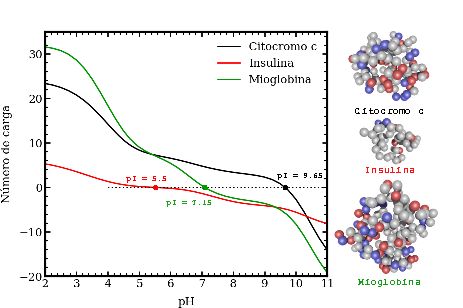
\includegraphics[width=0.65\textwidth]{Figures/graphs-gel2/protein-model.pdf}
     \caption{Izquierda: N\'umero de carga de las prote\'inas en una soluci\'on diluida en funci\'on del pH (curvas s\'olidas);
     	los c\'irculos llenos marcan el punto isoel\'ectrico,
     	donde la carga neta de la prote\'ina es cero.
     	La representaci\'on de grano grueso de las prote\'inas se ilustra a la derecha, donde los residuos de amino\'acidos se representan mediante una esfera \'unica (rojo: residuo \'acido; azul: residuo b\'asico; gris: residuos de carga neutral).}
     \label{fig:esf:protein-charge}
 \end{figure}



%%%%%%%%%%%%%%%%%%%%%%%%%%%%%%%%%%%%%%%%%%%%%%%%%%
\subsection{Modelo Molecular: Red polim\'erica}
%%%%%%%%%%%%%%%%%%%%%%%%%%%%%%%%%%%%%%%%%%%%%%%%%%

Adem\'as del modelo de prote\'ina presentado en la secci\'on anterior, necesitamos especificar un modelo molecular para describir la red que compone a nuestro nanogel. Este modelo debe proporcionar un conjunto representativo de configuraciones moleculares de la red polim\'erica. Una conformaci\'on particular de la red se da por la posici\'on espacial de todos sus segmentos.
La red del nanogel est\'a compuesta por cadenas polim\'ericas entrecruzadas de 25 segmentos de longitud. En total, esta red contiene 10054 segmentos. Cada segmento es una representaci\'on simplificada de una unidad neutra (VA), un mon\'omero \'acido/b\'asico (MAA/AH) o un segmento entrecruzante. La tabla \ref{table:Coarse-grain} incluye el volumen y el pKa (si la unidad es titulable) utilizados para describir estas unidades.

La red del nanogel posee una topolog\'ia tipo diamante, donde los segmentos entrecruzantes se colocan en la posici\'on original de los \'atomos de carbono. Los entrecruzantes se conectan a 4 cadenas polim\'ericas. La construcci\'on de esta red se realiz\'o en primera instancia por la traslaci\'on tridimensional de la celda unidad en donde todas las cadenas polim\'ericas se encuentran alargadas, como segundo paso se realiz\'o un corte esf\'erico de radio $R_{cut}$ medido desde el centro de masa de la estructura. El valor de $R_{cut}$ se hace de tal manera de obtener aproximadamente 10000 segmentos en total. 

Originalmente, todas las cadenas polim\'ericas se  conectan a dos entrecruzantes, pero como resultado de este procedimiento, el corte esf\'erico, algunas cadenas quedan lindantes en la superficie de la red, es decir  conectadas a un solo entrecruzante. La mayor\'ia de estas cadenas \emph{colgantes} superficiales son m\'as cortas que 25 segmentos. En conjunto, estas cadenas contienen el 22\% del n\'umero total de segmentos. Para generar las diferentes conformaciones moleculares de la red del pol\'imero, se ha realizado simulaciones de din\'amica molecular usando GROMACS 5.1.2 \cite{lindahl2001gromacs}.

 \begin{figure}[!htb]
     \centering
     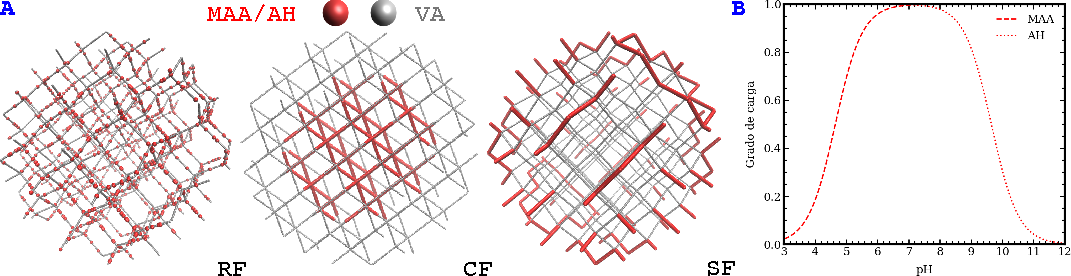
\includegraphics[width=0.99\textwidth]{Figures/graphs-gel2/ideal-charge-model.pdf}
     \caption{A: Los nanogeles estan formados por cadenas de copol\'imeros entrecruzadas con un segmento de carga neutral (VA: alcohol vin\'ilico) y una unidad funcional (ya sea MAA: \'acido metacr\'ilico o AH: alilamina).
     	Este esquema ilustra las tres distribuciones de los co-mon\'omeros consideradas; de izquierda a derecha: RF: una distribuci\'on aleatoria de grupos funcionales en toda la red; CF: las unidades funcionales ocupan el centro/n\'ucleo de la red; SF: solo las cadenas colgantes libres en la superficie de la red est\'an funcionalizadas con unidades sensibles al pH.
     	B: Gr\'afico del grado de carga ideal dependiente del pH de la unidad funcional aislada en soluci\'on diluida.}
     \label{fig:esf:gel-topologies}
 \end{figure}


 
 
 Consideramos diferentes nanogeles sensibles al pH que contienen grupos \'acidos (MAA) o b\'asicos (AH), y evaluamos tres topolog\'ias diferentes para la distribuci\'on espacial de estos segmentos funcionales, que se esquematizan en la Figura \ref{fig:esf:gel-topologies}:
 (i) una estructura \emph{aleatoriamente funcionalizada} ( Random Functionalization:  RF) donde los segmentos sensibles al pH se distribuyen aleatoriamente en toda la red,
 (ii) una estructura \emph{funcionalizada en el n\'ucleo} (Core Functionalization: CF), donde las unidades sensibles al pH ocupan el centro del nanogel, y
 (iii) una estructura \emph{funcionalizada en la superficie} (Surface Functionalization: SF) en la cual solo las cadenas colgantes en la superficie de la red son ionizables.
  







%%%%%%%%%%%%%%%%%%%%%%%%%%%%%%%%%%%%%%%%%%%%%%%%%%
\section{Resultados y discusi\'on}
%%%%%%%%%%%%%%%%%%%%%%%%%%%%%%%%%%%%%%%%%%%%%%%%%%






%%%%%%%%%%%%%%%%%%%%%%%%%%%%%%%%%%%%%%%%%%%%%%%%%%
\subsection{Caraterizaci\'on del nanogel}
%%%%%%%%%%%%%%%%%%%%%%%%%%%%%%%%%%%%%%%%%%%%%%%%%%

En esta primera instancia, se examinar\'a el comportamiento (la respuesta) de los nanogeles en funci\'on del pH en ausencia de prote\'inas.

Para cuantificar el tama\~no de un nanogel, utilizaremos el radio medio de la part\'icula, $R$, que se puede calcular utilizando la siguiente f\'ormula:
\begin{align}
	R = \frac{4}{3}\frac{\int_0^\infty{dr\,G(r)\,r \left<\phi(r)\right>}}{\int_0^\infty{dr\,G(r)\left<\phi(r)\right>}}
\end{align}
\noindent donde $r$ es la distancia desde el centro de masa de la red polim\'erica (como se ha mencionado en la secci\'on \ref{sec:esf:tm} se asume simetr\'ia radial);
$\left<\phi(r)\right>$ es la fracci\'on de volumen local de la red polim\'erica;
los corchetes angulares indican el promedio de ensamble sobre las diferentes conformaciones de la red (ver ecuaci\'on \ref{eq:esf:ensamble-gel});
$G(r)=4\pi r^2$ es el \'area de la superficie de una esfera de radio $r$.

\begin{figure}[!htb]
     \centering
     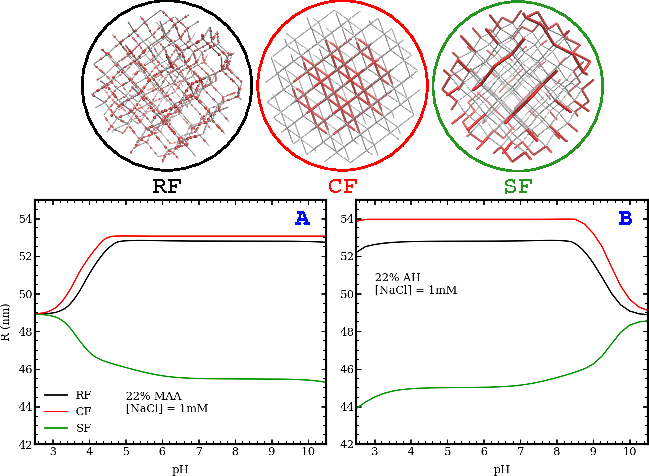
\includegraphics[width=0.65\textwidth]{Figures/graphs-gel2/rr-nano-pH.pdf}
     \caption{Radio promedio, R, en funci\'on del pH para nanogeles de copol\'imero MAA-VA (panel A) y AH-VA (panel B).
     	Se consideran tres estructuras diferentes en cada caso donde las unidades funcionales (MAA/AH) se distribuyen aleatoriamente a lo largo de la red polim\'erica (RF), ocupan el centro de la red (CF), o modifican las cadenas colgantes dentro del pol\'imero, interfaz de soluci\'on (SF).
     	En todos los casos, el $22\%$ de los segmentos de estas redes son sensibles al pH; La concentraci\'on de NaCl es $10^{-3}M$.}
     \label{fig:esf:gel-charge-MAA-AH}
\end{figure}


La Figura \ref{fig:esf:gel-charge-MAA-AH} muestra la relaci\'on entre el radio promedio ($R$) y el pH para las tres estructuras diferentes: RF, CF y SF. En el panel A, se describe un nanogel con segmentos ionizables de MAA, mientras que en el panel B se presenta un nanogel basado en AH. En ambos casos, la concentraci\'on de sal es de 1 mM y la fracci\'on de mon\'omero funcional (MAA o AH) es del $22\%$. Los nanogeles basados en MAA, funcionalizados al azar (RF) y en el n\'ucleo (CF), se hinchan a medida que aumenta el pH (panel A). Esto se debe a que los segmentos MAA se desprotonan y adquieren carga el\'ectrica a medida que el pH aumenta (ver Figura \ref{fig:esf:gel-topologies}B), lo que resulta en repulsiones electrost\'asticas dentro de la red. Para reducir estas interacciones repulsivas, la distancia entre las unidades cargadas de MAA debe aumentar, lo que provoca un aumento en el tama\~no de la red para separar estos segmentos cargados. En resumen, la expansi\'on neta de la red ocurre debido al aumento de la distancia espacial entre las unidades cargadas de MAA, como resultado de la necesidad de disminuir la repulsi\'on entre ellas.



Por otro lado, la red funcionalizada en su superficie con MAA muestra un comportamiento de expansi\'on completamente diferente, como se puede observar en la Figura \ref{fig:esf:gel-charge-MAA-AH}A. Este nanogel se deshincha a medida que las unidades titulables se cargan al aumentar el pH. Para explicar este comportamiento contrario a lo esperado, hemos examinado la distribuci\'on local de segmentos dentro de estas estructuras en diferentes condiciones. Hemos utilizado la distribuci\'on radial de los mon\'omeros funcionales para los nanogeles MAA. Esta cantidad se define como:



%
\begin{align}
    \lambda_{MAA}(r)= 4\pi r^2\left<\phi^{MAA}(r)\right>
\end{align}
%
\noindent en donde $\left<\phi_{MAA}(r)\right>$ da la fracci\'on de volumen local de los segmentos de \'acido metacr\'ilico (ver ecuaci\'on \ref{eq:esf:ensamble-gel})
Hay que tener en cuenta que $\lambda_{MAA}(r) dr$ da el n\'umero de segmentos MAA en la capa esf\'erica entre $r$ y $r+dr$ medido desde el centro del nanogel.
Adem\'as, la integral $\int_0^\infty \lambda_{MAA}(r) dr$ da el n\'umero total de mon\'omeros MAA en la red.


\begin{figure}[!htb]
     \centering
     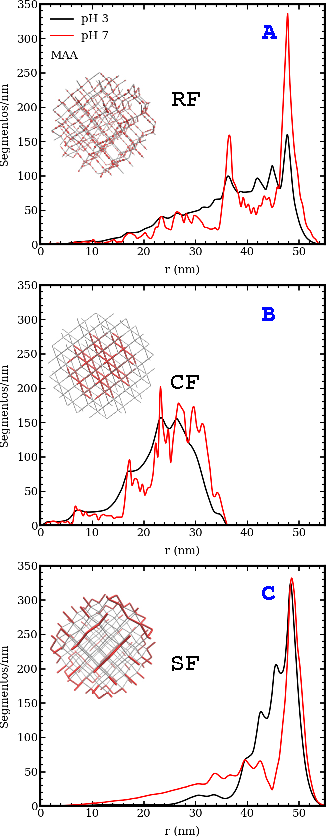
\includegraphics[width=0.30\textwidth]{Figures/graphs-gel2/dist-MAA.pdf}
     \caption{Distribuci\'on radial de segmentos MAA, $\lambda_{MAA}(r)$, a pH 3 y 7, y $10^{-3}M$ NaCl; cada panel corresponde a un nanogel de  MAA-VA diferente que tienen una funcionalizaci\'on de red particular y 22\% MAA.
     	Estos grupos funcionales est\'an completamente protonados (sin carga) a pH 3 y completamente disociados (cargados) a pH 7.}
     \label{fig:esf:MAA-vs-r-distribution}
 \end{figure}
 %\FloatBarrier

La Figura \ref{fig:esf:MAA-vs-r-distribution} muestra la distribuci\'on radial de los segmentos de MAA para las diferentes redes consideradas. En cada caso, se incluyen resultados para una soluci\'on de pH 3, donde los segmentos MAA tienen carga neutra, y pH 7, donde est\'an completamente cargados (ver Figura \ref{fig:esf:gel-topologies}B). Para una funcionalizaci\'on de tipo aleatoria (Panel A), la distribuci\'on de los segmentos MAA se desplaza hacia la interfaz de soluci\'on del nanogel a medida que la red se carga el\'ectricamente al aumentar el pH. Este desplazamiento ocurre para reducir las repulsiones electrost\'aticas entre los segmentos MAA cargados.

Como resultado, toda la distribuci\'on del pol\'imero tambi\'en se extiende, incluidas las unidades VA de carga neutra (ver Figura \ref{fig:esf:allr-distribution}). El mismo comportamiento tiene lugar para una funcionalizaci\'on central (Panel B), aunque por dise\~no, los segmentos MAA en esta red, ya sea que est\'en cargados o no, es m\'as probable que ocurran a distancias m\'as cortas del centro del nanogel en comparaci\'on con las otras estructuras. El desplazamiento de segmentos a valores m\'as altos de $r$ observado en los paneles A y B de la Figura \ref{fig:esf:MAA-vs-r-distribution} explica el aumento del tama\~no promedio del nanogel con pH observado en la Figura \ref{fig:esf:gel-charge-MAA-AH}A para las estructuras RF y CF.

Por otro lado, la Figura \ref{fig:esf:MAA-vs-r-distribution}C muestra que la distribuci\'on superficial de segmentos de MAA se desplaza hacia el interior cuando la red se carga con el aumento de pH. Para reducir las repulsiones dentro de la red, las cadenas libres (de la superficie) de PMAA, que se asientan en la superficie del nanogel a un pH bajo, tambi\'en intentan ocupar el volumen dentro de la red cuando est\'an cargadas. Este desplazamiento hacia el interior de la distribuci\'on de pol\'imero (Figura \ref{fig:esf:allr-distribution}C) explica el comportamiento de compresi\'on del nanogel tipo SF con el aumento del pH observado en la Figura \ref{fig:esf:gel-charge-MAA-AH}A. N\'otese, sin embargo, que a pesar de este desplazamiento parcial hacia el interior de la red, la posici\'on m\'as probable de los segmentos MAA siempre es la interfaz pol\'imero-soluci\'on para soluciones de pH alto y bajo. Al empujar toda la estructura hacia el interior del nanogel, los segmentos de MAA quedan igualmente expuestos a la soluci\'on



El comportamiento de los nanogeles compuestos por AH es an\'alogo al de las redes basadas en MAA, pero en respuesta al cambio de pH en la direcci\'on opuesta.
Los grupos AH se protonan y se cargan positivamente con la disminuci\'on del pH (ver figura \ref{fig:esf:gel-topologies}B).
Para nanogeles de AH funcionalizados aleatoriamente y en su n\'ucleo, este aumento en la carga el\'ectrica con la disminuci\'on del pH provoca un desplazamiento hacia afuera de la distribuci\'on del segmento. Del mismo modo que se observ\'o para los nanogeles compuestos por MAA% (ver \cref*{fig:AHseg_si}A y B)
, lo que explica la expansi\'on observada en la figura \ref{fig:esf:gel-charge-MAA-AH}B;
mientras tanto, para la estructura tipo SF, el deswelling con la disminuci\'on del pH (figura \ref{fig:esf:gel-charge-MAA-AH}B) es consistente con un desplazamiento hacia adentro del pol\'imero %(ver \cref*{fig:AHseg_si}C) .


La figura \ref{fig:esf:allr-distribution} muestra la distribuci\'on de todos los segmentos que componen la red polim\'erica de los diferentes nanogeles. 
Al igual que en la figura \ref{fig:esf:MAA-vs-r-distribution} presentamos la distribuci\'on para dos diferentes valores de pH. Que corresponden a los estados protonado (pH 3) y desprotonado (pH 7) de los segmentos de MAA.  En los paneles A y B se observa un mayor n\'umero de segmentos a valores m\'as altos de $r$ al cargarse el nanogel. Observ\'andose el swelling reportado en la figura \ref{fig:esf:gel-charge-MAA-AH}A para lo nanogeles tipo RF y CF.
En cambio, el desplazamiento hacia dentro de los segmentos de la red polim\'erica al transicionar de un estado cargado a uno descargado en la distribuci\'on superficial (SF) (figura \ref{fig:esf:allr-distribution}C) explica la disminuci\'on del tama\~no del nanogel observada en la figura \ref{fig:esf:gel-charge-MAA-AH}A.

El comportamiento de los nanogeles compuestos por AH es an\'alogo al de las redes basadas en MAA, pero en respuesta al cambio de pH en la direcci\'on opuesta. Los grupos AH se protonan y se cargan positivamente con la disminuci\'on del pH (ver Figura \ref{fig:esf:gel-topologies}B). Para nanogeles de AH funcionalizados aleatoriamente y en su n\'ucleo, este aumento en la carga el\'ectrica con la disminuci\'on del pH provoca un desplazamiento hacia afuera de la distribuci\'on del segmento, similar a lo observado para los nanogeles compuestos por MAA. Esto explica la explicaci\'on del nanogel  observada en la Figura \ref{fig:esf:gel-charge-MAA-AH}B. Por otro lado, para la estructura tipo SF, la disminuci\'on del tama\~no del nanogel  con la disminuci\'on del pH que se observa en la Figura \ref{fig:esf:gel-charge-MAA-AH}B es consistente con un desplazamiento de los segmentos que componen la red hacia el interior del nanogel.% (ver Figura \ref{fig:AHseg_si}C).

En la figura \ref{fig:esf:allr-distribution} se muestra la distribuci\'on de todos los segmentos que componen la red polim\'erica de los diferentes nanogeles (en este caso basados en MAA). Al igual que en la Figura \ref{fig:esf:MAA-vs-r-distribution}, presentamos la distribuci\'on para dos valores diferentes de pH, correspondientes a los estados protonado (pH 3) y desprotonado (pH 7) de los segmentos de MAA. En los paneles A y B se observa un aumento en la cantidad de segmentos a valores m\'as altos de $r$ a medida que el nanogel se carga el\'ectricamente. Este comportamiento es consistente con el aumento del radio del nanogel observado en la figura \ref{fig:esf:gel-charge-MAA-AH} para las estructuras RF y CF. Por otro lado, el desplazamiento hacia el interior de los segmentos de la red polim\'erica al transicionar de un estado cargado a uno descargado en la distribuci\'on superficial (SF) explica la disminuci\'on del tamañ\~no del nanogel observada en la figura \ref{fig:esf:gel-charge-MAA-AH}B.

\begin{figure}[!htb]
	\centering
	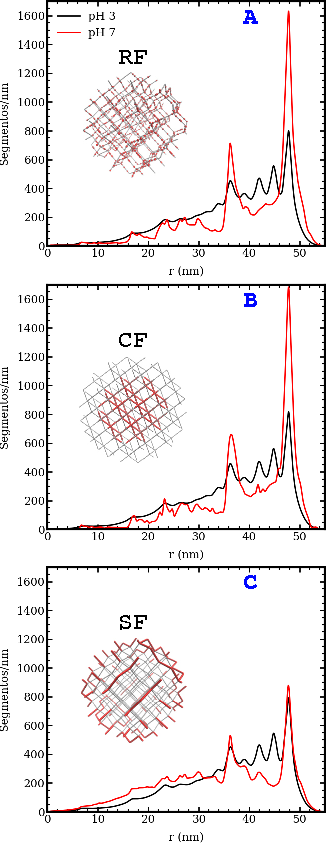
\includegraphics[width=0.30\textwidth]{Figures/graphs-gel2/allseg_SI.pdf}
	\caption{Distribuci\'on radial de todos los segmentos que componen la estructura del nanogel a pH 3 y 7, y $10^{-3}M$ NaCl; cada panel corresponde a una funcionalizaci\'on  diferente de la red polim\'erica.}
	\label{fig:esf:allr-distribution}
\end{figure}




%%%%%%%%%%%%%%%%%%%%%%%%%%%%%%%%%%%%%%%%%%%%%%%%%%
\subsection{Adsorci\'on de prote\'inas en nanogeles basados en MAA}\label{sec:MAA-NGs}
%%%%%%%%%%%%%%%%%%%%%%%%%%%%%%%%%%%%%%%%%%%%%%%%%%



%%%%%%%%%%%%%%%%%%%%%%%%%%%
%%%%% Define Gamma and N(r)
%%%%%%%%%%%%%%%%%%%%%%%%%%%



En la secci\'on anterior, se evalu\'o el impacto de la funcionalizaci\'on de la red y la composici\'on qu\'imica en la respuesta del nanogel a las variaciones de pH en ausencia de prote\'inas. La reorganizaci\'on de los segmentos de la red polim\'erica es resultado de los cambios en el pH, con una dependencia en la elecci\'on de dise\~no, es decir, la distribuci\'on de unidades funcionales dentro de la red.

En esta parte, se mostrar\'a el impacto de esta reorganizaci\'on de la red polimé\'erica en el nivel de adsorci\'on de prote\'inas en diferentes nanogeles, as\'i como la distribuci\'on espacial de las prote\'inas adsorbidas. En particular, se presentar\'a el an\'alisis de la adsorci\'on del citocromo c y mioglobina en las diferentes estructuras de nanogeles basados en MAA. Adem\'as, se realizar\'an estudios de adsorci\'on de insulina, pero en este caso con nanogeles que contienen AH como segmento protonable.% Los resultados de la insulina con MAA se omiten debido a su bajo punto isoel\'ectrico, ya que esta prote\'ina no se adsorbe en nanogeles basados en $MAA$.

Para estos estudios, se considerar\'a un nanogel polim\'erico  con centro de masa centrado en $r=0$ en contacto con una soluci\'on acuosa de prote\'ina con concentraci\'on definida. El n\'umero de prote\'inas adsorbidas dentro de la capa esf\'erica entre $r$ y $r+dr$ se define como la cantidad en exceso. 


\begin{align}
     \langle N(r)\rangle dr = 4\pi r^2 \left(\langle\rho(r)\rangle - \rho_{bulk}\right) dr
\end{align}
%
en donde $\left<\rho(r)\right>$ y $\rho^b_{pro}=\lim\limits_{r\to \infty } \langle\rho(r)\rangle$ son respectivamente la densidad (en n\'umero) local y en el bulk de la prote\'ina.
La integraci\'on de $\langle N(r)\rangle$ produce la \emph{adsorci\'on en exceso} (en adelante, simplemente la adsorci\'on) que cuantifica el n\'umero de prote\'inas incorporadas a la red polim\'erica,


%
\begin{align}
    \Gamma =  \int_0^\infty{  \langle N(r)\rangle dr}
\end{align}
%

%%%%%%%%%%%%%%%%%%%%%%%%%%%
%%%%% Adsorption to MAA NGs
%%%%%%%%%%%%%%%%%%%%%%%%%%%


\begin{figure}[!htb]
	\centering
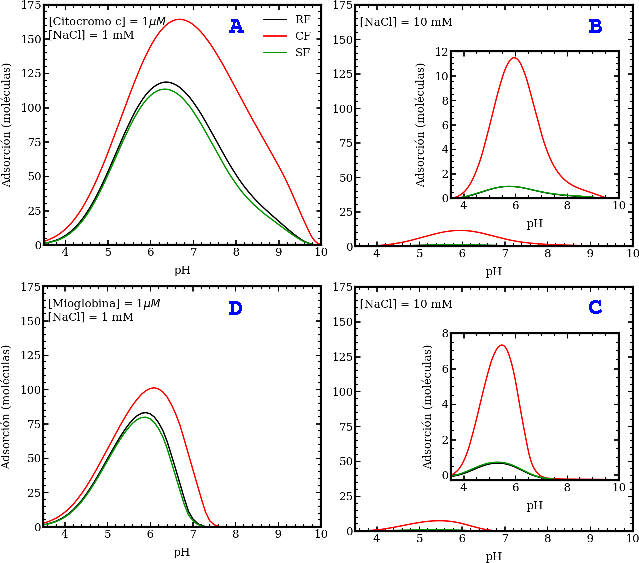
\includegraphics[width=0.75\textwidth]{Figures/graphs-gel2/ad-maa-pH-proteins.pdf}
\caption{Gr\'aficos de la adsorci\'on en exceso $\Gamma$ de citocromo c (paneles A y B) y mioglobina (paneles C y D) a nanogeles MAA-VA en funci\'on del pH.
	La concentraci\'on de sal es $10^{-3}M$ en los paneles de la izquierda (A y C) y $10^{-2}M$ en los paneles de la derecha
	(B y D);  En los paneles B y C Se muestra en el inset un zoom de la adsorci\'on.
	Estos nanogeles tienen 22\% MAA; la concentraci\'on de prote\'ina es $10^{-6}M$ en cada caso.}
\label{fig:esf:adsorption-vs-pH-cyto-myo}
\end{figure}
 
 La Figura \ref{fig:esf:adsorption-vs-pH-cyto-myo} muestra la adsorci\'on de soluciones, en diluci\'on infinita, de citocromo c (paneles superiores, A y B) y mioglobina (paneles inferiores, C y D) en nanogeles de MAA-VA con diferentes funcionalizaciones en su red. El pH se utiliz\'o como variable independiente en estos c\'alculos, y tambi\'en se evalu\'o el efecto de la concentraci\'on de NaCl al comparar diferentes paneles en la misma l\'inea. Los nanogeles de la Figura \ref{fig:esf:adsorption-vs-pH-cyto-myo} contienen un $22\%$ de MAA, lo que implica que todos los segmentos en las cadenas superficiales de la red son MAA.
 
 Se puede observar que la adsorci\'on de prote\'inas muestra un comportamiento no monot\'onico en funci\'on del pH, alcanzando un m\'aximo en la regi\'on entre pH 5 y 7. Este comportamiento est\'a influenciado por la concentraci\'on de sal y la prote\'ina espec\'ifica considerada. Esta respuesta se puede explicar mediante las interacciones electrost\'aticas y el comportamiento de protonaci\'on de los segmentos de MAA y de las prote\'inas. A medida que el pH aumenta por encima del pKa intr\'inseco de MAA (4.65), las unidades \'acidas del pol\'imero se disocian, cargando negativamente la red. Por encima del pKa del MAA, pero por debajo del punto isoel\'ectrico de cada prote\'ina, esta adquieren carga positiva. En estas condiciones, las interacciones atractivas entre las prote\'inas y la red polim\'erica promueven la adsorci\'on. Sin embargo, en ambos extremos de la escala de pH, estas interacciones son bajas: a pH bajo, el MAA est\'a protonado y tiene carga neutra, mientras que a pH alto, las prote\'inas tienen carga negativa. En ambos casos, esto conduce a una ausencia de adsorci\'on ($\Gamma \approx 0$) o incluso a una desorci\'on ($\Gamma < 0$).
 
 
En general, la adsorci\'on de citocromo c y la de mioglobina son cualitativamente similares. Sin embargo, existen dos diferencias principales: (i) la magnitud de la adsorci\'on ,el citocromo c se adsorbe significativamente m\'as y (ii) el rango de pH en el que ocurre la adsorci\'on (el citocromo c se adsorbe en un rango de pH m\'as amplio debido a su punto isoel\'ectrico m\'as alto, 9.65 en comparaci\'on con 7.15 para la mioglobina). Esto implica que, bajo condiciones similares, el nivel m\'aximo de adsorci\'on de citocromo c se alcanza a un pH ligeramente m\'as alto.

En cuanto a las otras configuraciones, la Figura \ref{fig:esf:adsorption-vs-pH-cyto-myo} muestra que la distribuci\'on central de los segmentos MAA conduce a una adsorci\'on significativamente mayor en la mayor\'ia de las condiciones. Este comportamiento se debe a que dicha distribuci\'on de segmentos MAA permite una incorporaci\'on m\'as efectiva de la prote\'ina adsorbida con carga el\'ectrica opuesta. Por otro lado, el comportamiento de adsorci\'on en las redes funcionalizadas aleatoriamente y en la superficie es sorprendentemente similar en el rango de pH y concentraciones de sal estudiadas, tanto para las diferentes prote\'inas como entre s\'i. Aunque las distribuciones de unidades funcionales entre las estructuras RF y SF difieren significativamente a pH bajo, se vuelven relativamente similares entre s\'i despu\'es de la reorganizaci\'on del nanogel a un pH m\'as alto cuando las unidades MAA se cargan. Esto explica la adsorci\'on comparable de prote\'inas observada en los nanogeles RF y SF (comparece los paneles A y C de la Figura \ref{fig:esf:MAA-vs-r-distribution}).



%%%%%%%%%%%%%%%%%%%%%%%%%%
%%%%% Protein localization
%%%%%%%%%%%%%%%%%%%%%%%%%%

\begin{figure}[!htb]
     \centering
     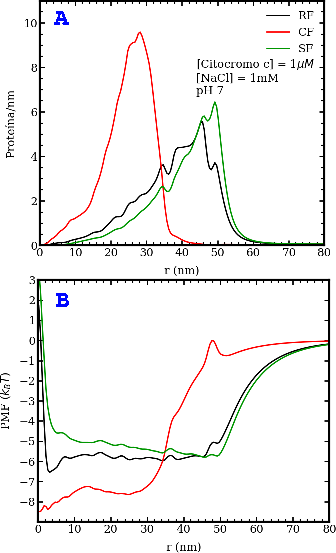
\includegraphics[width=0.40\textwidth]{Figures/graphs-gel2/cito-adsr-pmf.pdf}
     \caption{Panel A: Gr\'afico de la distribuci\'on radial de las mol\'eculas de citocromo c, $\langle N(r)\rangle$, en funci\'on de su posici\'on, para los nanogeles MAA-VA con diferentes funcionalizaciones.
     	Estas part\'iculas tienen 22\% MAA, el pH es 7, la concentraci\'on de prote\'ina es de $10^{-6}M$ y la concentraci\'on de NaCl es de $10^{-3}M$.
     	El panel B muestra el potencial de la fuerza media, ${PMF}(r)$, que act\'ua sobre el citocromo c para las mismas condiciones que el panel A.}
     \label{fig:esf:adsorption-vs-r-cyto}
 \end{figure}



Para explicar el mejor rendimiento de los nanogeles MAA funcionalizados en su n\'ucleo para la incorporaci\'on de prote\'inas, se muestra en la Figura \ref{fig:esf:adsorption-vs-r-cyto}A la distribuci\'on radial de las mol\'eculas de citocromo c en funci\'on de la distancia $r$ al centro de masa del nanogel. La soluci\'on tiene un pH de 7 y una concentraci\'on de NaCl de $1 $ mM, que corresponden aproximadamente a las condiciones de m\'axima adsorci\'on de esta prote\'ina en la Figura \ref{fig:esf:adsorption-vs-pH-cyto-myo}A. Existe una clara correlaci\'on entre la distribuci\'on de los grupos funcionales a lo largo de la red polim\'erica y la ubicaci\'on del citocromo c adsorbido.

Cuando el centro de la red est\'a funcionalizado, la mayor probabilidad de encontrar las prote\'inas ocurre en el interior del nanogel, entre 20 y 30 nm. En la figura \ref{fig:esf:adsorption-vs-r-cyto}A, el n\'umero m\'aximo de prote\'inas adsorbidas se produce a $r=28$ nm para 1 mM de NaCl. Coherentemente, el perfil de distribuci\'on de los grupos MAA cargados muestra un m\'aximo suave en esta regi\'on espacial (ver Figura \ref{fig:esf:MAA-vs-r-distribution}B, curva roja). Es decir, las prote\'inas adsorbidas se ubican donde pueden estar rodeadas de segmentos de la red con carga el\'ectrica opuesta. Curiosamente, el mismo fen\'omeno ocurre en la adsorci\'on a los nanogeles RF y SF. Las distribuciones de MAA cargados muestran un m\'aximo pronunciado cerca de la superficie del nanogel, entre 45 y 50 nm (ver curvas rojas en la figura \ref{fig:esf:MAA-vs-r-distribution}, paneles A y C). La figura \ref{fig:esf:adsorption-vs-r-cyto}A muestra que el citocromo c se adsorbe preferentemente en estas regiones de alta densidad de MAA, y por ende una alta densidad de carga el\'ectrica.



Al comparar las distribuciones de citocromo c dentro de los nanogeles RF y SF en la Figura \ref{fig:esf:adsorption-vs-r-cyto}A, observamos que los perfiles son relativamente similares entre s\'i. Como era de esperar, si solo se funcionaliza la superficie, el perfil de la prote\'ina se desplaza hacia la interfaz pol\'imero-soluci\'on.

Para cuantificar a\'un m\'as la interacci\'on con los nanogeles, utilizamos el potencial de fuerza media (PMF) que act\'ua sobre una prote\'ina a una distancia $r$ desde el centro de la red polim\'erica. El PMF se define como:

\begin{align}
	\text{PMF}(r) = -k_B T \ln \frac{\langle \rho(r)\rangle}{\rho_{\text{bulk}}}
\end{align}

donde $\lim\limits_{r\to \infty}\text{PMF}(r)=0$, lo que indica que la interacci\'on nanogel-prote\'ina desaparece cuando est\'an suficientemente lejos.

La Figura \ref{fig:esf:adsorption-vs-r-cyto}B muestra el PMF que act\'ua sobre el citocromo c en las mismas condiciones que en el panel A, pero para las tres diferentes funcionalizaciones de nanogeles. En el interior del nanogel, la interacci\'on de la prote\'ina con la estructura CF es la m\'as fuerte, aproximadamente $-8k_B T$ en el rango espacial de $r=0$ a 30 nm. Esta interacci\'on es de relativo corto alcance, ya que disminuye significativamente por encima de $r > 40$ nm.

Por otro lado, las interacciones del citocromo c con los nanogeles RF y SF se extienden m\'as lejos, hasta $55-60$ nm. En el interior del nanogel, estas interacciones son m\'as d\'ebiles que aquellas de la estructura CF. La energ\'ia libre de adsorci\'on es aproximadamente $-6 k_BT$, y se mantiene casi constante dentro del nanogel RF.

Para el nanogel funcionalizado en la superficie, sin embargo, el m\'inimo del PMF tambi\'en es de alrededor de $-6 k_BT$, y ocurre junto a la interfaz pol\'imero-soluci\'on a $r\approx 50$ nm. A diferencia de la estructura RF, esta interacci\'on no es constante dentro del nanogel. 

%En cambio, aumenta de manera monot\'onica a medida que $r$ disminuye, lo que indica que la prote\'ina se aleja de las cadenas superficiales funcionalizadas y se ubica m\'as profundamente en el nanogel.



%%%%%%%%%%
%%%% change in salt

\begin{figure}[!htb]
     \centering
     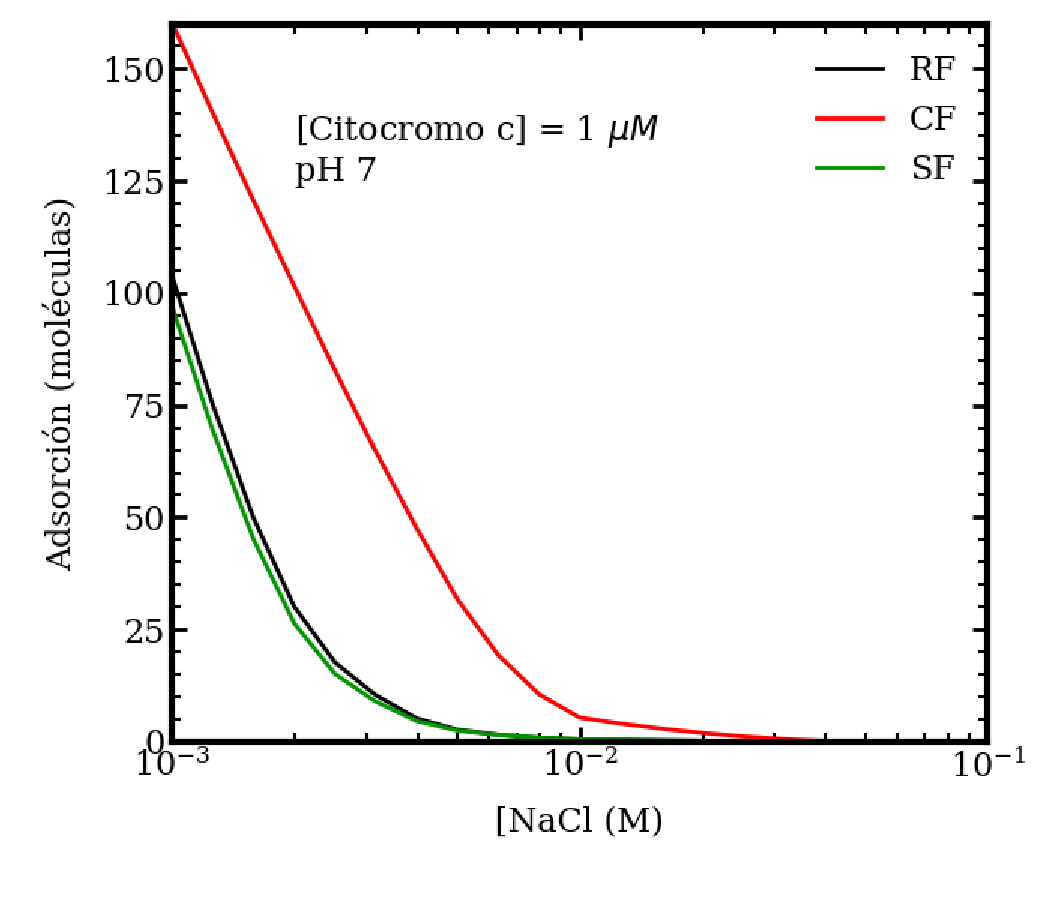
\includegraphics[width=0.45\textwidth]{Figures/graphs-gel2/gamma-salts-cito.pdf}
     \caption{Gr\'afico de la adsorci\'on en exceso $\Gamma$ del citocromo c en funci\'on de la concentraci\'on de sal a pH 7 para nanogeles MAA-VA con diferentes funcionalizaciones de red que contienen un 22\% de MAA; la concentraci\'on de prote\'ina es de $10^{-6}M$.}
     \label{fig:esf:adsorption-vs-salt-cyto}
 \end{figure}
 

Una caracter\'istica de la adsorci\'on de prote\'inas que nos falta discutir es el efecto de la concentraci\'on de sal.
Tanto para el citocromo c como para la mioglobina, la figura \ref{fig:esf:adsorption-vs-pH-cyto-myo} muestra que la incorporaci\'on de prote\'inas dentro de los diferentes nanogeles se ve significativamente mejorada al disminuir la concentraci\'on de sal en la soluci\'on.
Para caracterizar mejor este comportamiento, la figura \ref{fig:esf:adsorption-vs-salt-cyto} presenta la adsorci\'on de citocromo c en funci\'on de la concentraci\'on de NaCl a pH 7.
Este gr\'afico muestra que todas las funcionalizaciones de la red presentan un comportamiento cualitativamente similar, con una disminuci\'on dr\'astica en la adsorci\'on entre 1 y 10 mM de NaCl.
A 100 mM, todos los nanogeles muestran una adsorci\'on cercana a cero o negativa, dado que es una adsorci\'on por exceso esto \'ultimo significa que hay menos prote\'ina en el interior del nanogel que en la soluci\'on bulk.

Cuando la concentraci\'on de sal en la soluci\'on es alta, tanto los iones Na$^+$ como los iones Cl$^-$ se encuentran en altas concentraciones dentro del nanogel.
Estos iones opacan las atracciones electrost\'aticas entre las cargas positivas de la prote\'ina y las cargas negativas del nanogel, que son la fuerza impulsora para la adsorci\'on de prote\'inas.
En efecto, estas atracciones se vuelven de corto alcance y no son lo suficientemente fuertes como para dar lugar a una adsorci\'on significativa, de ocurrir dicho fen\'omeno.
Por otro lado, si la concentraci\'on de NaCl es menor, estas interacciones electrost\'aticas se ven menos apantalladas y efectivamente tienen un alcance mayor, lo que favorece la adsorci\'on de prote\'inas.
Por lo tanto, la disminuci\'on de la concentraci\'on de sal mejora la adsorci\'on.
Este comportamiento ha sido observado en experimentos; los brushes  de  polielectrol\'iticos muestran un aumento en la adsorci\'on de prote\'inas a baja concentraci\'on de sal \cite{wittemann2006interaction,becker2012proteins, henzler2010adsorption,xu2018interaction}.

Al considerar veh\'iculos para aplicaciones de liberaci\'on de prote\'inas, nuestros resultados sugieren que las mejores condiciones para la encapsulaci\'on corresponden a una baja concentraci\'on de sal.
Los perfiles de adsorci\'on de la figura \ref{fig:esf:adsorption-vs-salt-cyto} son cualitativamente similares para las tres funcionalizaciones, pero el n\'umero de prote\'inas dentro del nanogel siempre es significativamente mayor para la estructura CF.
Esta caracter\'istica puede ser cr\'itica en el dise\~no de veh\'iculos de liberaci\'on para un objetivo que tenga una concentraci\'on de sal intermedia.
El CF incorpora m\'as prote\'inas en las mismas condiciones, pero puede no ser capaz de liberarlas si el objetivo tiene una concentraci\'on de sal intermedia.
Para estas condiciones, la funcionalizaci\'on aleatoria podr\'a liberar toda su carga.



%%%%%%%%%%%%%%%%%%%%%%%%%%%%%%%%%%%%%%%%%%%%%%%%%%
\subsection{Adsorci\'on de insulina en nanogeles basados en  AH} 
%%%%%%%%%%%%%%%%%%%%%%%%%%%%%%%%%%%%%%%%%%%%%%%%%%

La insulina no se adsorbe a los nanogeles de MAA de la secci\'on \ref{sec:MAA-NGs} %(ver \cref*{fig:adsoprtion-vs-pH-insulinMAA_si} en SI).
Esto se debe a que el punto isoel\'ectrico de la insulina y el pKa del MAA est\'an cerca entre s\'i (5.5 y 4.65 respectivamente), lo que significa que para soluciones donde la prote\'ina tiene carga positiva, el nanogel tiene carga neutra, y si el nanogel tiene carga negativa, tambi\'en la tiene la prote\'ina.
En este contexto, se investiga la adsorci\'on de insulina en un nanogel de alilamina, que tiene carga positiva por debajo de su pKa de 9.5, superponi\'endose con el rango donde la insulina tiene carga negativa.
Aparte de los mon\'omeros funcionales, la estructura de estas redes de copol\'imero AH-VA es la misma que la de los nanogeles de MAA-VA descritos anteriormente.


\begin{figure}[!htb]
    \centering
    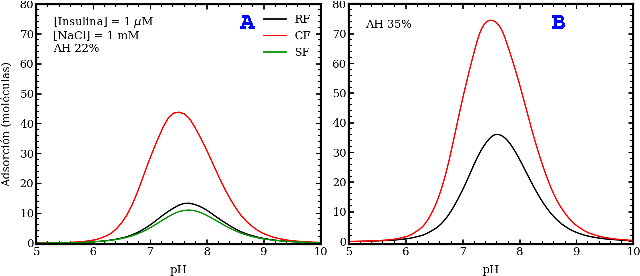
\includegraphics[width=0.75\textwidth]{Figures/graphs-gel2/insu-PAH.pdf}
    \caption{Gr\'aficos de las mol\'eculas de insulina adsorbidas, $\Gamma$, en funci\'on del pH para nanogeles AH-VA con diferentes funcionalizaciones.
    	El contenido de AH es del 22\% para las redes polim\'ericas del panel A y del 35\% para las del panel B (este \'ultimo grado de funcionalizaci\'on no se alcanza para el nanogel SF).
    	 La concentraci\'on de sal es $10^{-3}$ M de NaCl y [Insulina] = $10^{-6}$ M.}
    \label{fig:esf:adsorption-vs-pH-insulin}
\end{figure}




La figura \ref{fig:esf:adsorption-vs-pH-insulin}A muestra la adsorci\'on de insulina en nanogeles basados en AH con diferentes funcionalizaciones espaciales.
Una vez m\'as, hemos considerado redes con un $22\%$ de mon\'omeros sensibles al pH para poder incluir resultados para el nanogel SF, cuyas cadenas colgantes estan completamente compuestas  de AH. 
Las principales caracter\'isticas de este gr\'afico son cualitativamente similares a las de la adsorci\'on de citocromo c y mioglobina en los nanogeles de MAA (ver figura \ref{fig:esf:adsorption-vs-pH-cyto-myo}).
Es decir, la insulina muestra una adsorci\'on no monot\'onica en funci\'on del pH de la soluci\'on.
Adem\'as, observamos que la distribuci\'on central de los segmentos de AH captura m\'as insulina que las funcionalizaciones aleatorias o superficiales.
Los nanogeles RF y SF muestran perfiles de adsorci\'on dependientes del pH relativamente similares.
Finalmente, una mayor concentraci\'on de sal tiene un efecto cr\'itico en la magnitud de la adsorci\'on de insulina, que disminuye significativamente debido al aumento del apantallamiento de las atracciones electrost\'aticas entre la red y la prote\'ina por los iones m\'oviles
%(las curvas de adsorción para $10^{-2}$,M de NaCl se pueden ver en la figura \ref{fig:esf:adsoprtion-AH-1d-2-insu_si}).

La figura \ref{fig:esf:adsorption-vs-pH-insulin}A muestra que los nanogeles basados en AH son efectivos para encapsular insulina.
Sin embargo, a pesar de las similitudes cualitativas entre los perfiles de adsorci\'on de esta figura y los de citocromo c y mioglobina (\ref{fig:esf:adsorption-vs-pH-cyto-myo}A y C), vemos que la cantidad de mol'eculas de insulina capturadas por los nanogeles de AH es significativamente menor que la de las otras prote\'inas capturadas por los nanogeles basados en MAA.
Por esta raz\'on, tambi\'en hemos evaluado el efecto del grado de funcionalizaci\'on de la red de pol\'imero para mejorar la adsorci\'on de prote\'inas.
La figura \ref{fig:esf:adsorption-vs-pH-insulin}B presenta la adsorci\'on de insulina para nanogeles con un $35\%$ de segmentos de AH.
En este caso, la estructura funcionalizada en la superficie no se incluye porque no hay suficientes segmentos en las cadenas colgantes para llegar a ese porcentaje.
Un mayor contenido de AH promueve una mayor adsorci\'on, como se puede observar al comparar ambos paneles de la figura \ref{fig:esf:adsorption-vs-pH-insulin}.
Una vez m\'as, el nanogel CF adsorbe m\'as insulina que la red RF (m\'as del doble de prote\'inas para las condiciones de estos c\'alculos).




\begin{figure}[!htb]
    \centering
    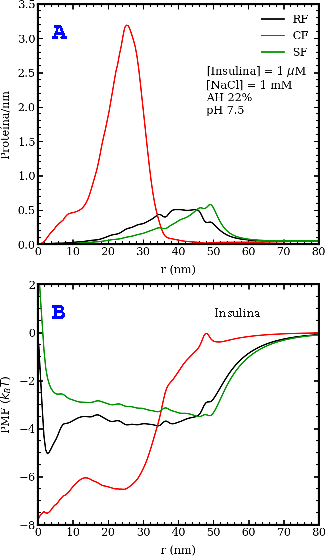
\includegraphics[width=0.40\textwidth]{Figures/graphs-gel2/insu-ads-pmf.pdf} 
    \caption{A: Gr\'afico de la distribuci\'on local de mol\'eculas de insulina, $\langle N(r) \rangle$, en funci\'on de la posici\'on para nanogeles AH-VA con un 22\% de segmentos sensibles al pH en diferentes configuraciones de red.
    	El pH es 7.5, la concentraci\'on de insulina es de $10^{-6}$ M y la de NaCl es de $10^{-3}$ M.
    	B: Potencial de fuerza media, ${PMF}(r)$ actuando sobre la prote\'ina, en funci\'on de la posici\'on para las mismas condiciones que el panel A.}
    \label{fig:esf:adsorption-vs-r-insulin}
\end{figure}



A continuaci\'on, describimos la distribuci\'on de mol\'eculas de insulina dentro de los nanogeles basados en AH.
La figura \ref{fig:esf:adsorption-vs-r-insulin}A muestra c\'omo se disponen espacialmente las prote\'inas adsorbidas dentro de los diferentes nanogeles basados en AH con un grado de funcionalizaci\'on del $22\%$;
utilizamos ese grado de funcionalizaci\'on para comparar los resultados de los nanogeles CF, RF y SF.
El pH de estos resultados corresponde al m\'aximo de adsorci\'on de la figura \ref{fig:esf:adsorption-vs-pH-insulin}A.
La adsorci\'on de insulina en el nanogel CF no solo es significativamente mayor que la adsorci\'on en los nanogeles RF y SF, sino que tambi\'en ocurre en una posici\'on m\'as profunda dentro de la estructura.
La posici\'on m\'as probable de una mol\'ecula de insulina se encuentra alrededor de $r=25$ nm para el nanogel CF,
mientras que esta posici\'on se desplaza a alrededor de 40-45 y 50 nm para las estructuras RF y SF, respectivamente.

Para los nanogeles basados en MAA, la figura \ref{fig:esf:adsorption-vs-r-cyto}A muestra diferencias relativamente menores entre las distribuciones de citocromo c en los nanogeles RF y SF.
Estas diferencias se acent\'uan ligeramente al observar la adsorci\'on de insulina en los nanogeles AH-VA, como se muestra en la figura \ref{fig:esf:adsorption-vs-r-insulin}A.
La distribuci\'on de insulina se desplaza hacia el interior de la red en el nanogel modificado aleatoriamente en comparaci\'on con la funcionalizaci\'on superficial, donde las prote\'inas tienen m\'as probabilidades de ocupar la vecindad inmediata de la interfaz nanogel-soluci\'on.
Los perfiles de distribuci\'on de insulina siguen siendo relativamente similares para estas dos estructuras.

El panel B de la figura \ref{fig:esf:adsorption-vs-r-insulin} muestra el potencial de fuerza media que act\'ua sobre las mol\'eculas de insulina en las mismas condiciones que el panel A.
La interacci\'on atractiva en la insulina adsorbida var\'ia desde $-8$ hasta $-6 k_B T$ en el interior de la estructura CF y desde $-5$ hasta $-4 k_B T$ en el nanogel RF.
En el nanogel SF, el potencial presenta un m\'inimo de $-4 k_B T$ en la superficie y luego aumenta mon\'otonamente a medida que $r$ disminuye dentro del gel.
En general, los resultados de esta secci\'on muestran, una vez m\'as, que el dise\~no de la red (mediante la s\'intesis del nanogel) proporciona una herramienta para controlar la distribuci\'on y localizaci\'on de prote\'inas dentro del nanogel.






%%%%%%%%%%%%%%%%%%%%%%%%%%%%%%%%%%%%%%%%%%%%%%%%%%
\section{Conclusiones}
%%%%%%%%%%%%%%%%%%%%%%%%%%%%%%%%%%%%%%%%%%%%%%%%%%


En este cap\'itulo investigamos la adsorci\'on de prote\'inas en nanogeles polim\'ericos con diferentes funcionalizaciones espaciales y sensibles al pH. Se desarroll\'o y aplic\'o una teor\'ia termodin\'amica basada en un modelo molecular.
El enfoque se centr\'o en la influencia de las interacciones electrost\'aticas, por lo cual se describieron tres prote\'inas con diferentes puntos isoel\'ectricos (insulina, mioglobina y citocromo c) utilizando un modelo molecular basado en sus estructuras cristalogr\'aficas.
Exploramos las propiedades de los nanogeles sensibles al pH modificados con m\'onomeros de  \'acido metacr\'ilico o de alilamina.
Se consideraron tres configuraciones diferentes, con los segmentos sensibles al pH distribuidos al azar, en el centro o en la superficie de la red del nanogel.

Se examin\'o el comportamiento de estos nanogeles en funci\'on del pH cuando no hay prote\'inas presentes en la soluci\'on.
Los resultados muestran que, para los nanogeles basados en \'acido metacr\'ilico, tanto los estructurados con distribuci\'on distribuidos al azar como los funcionalizados en el n\'ucleo se expanden con el aumento del pH, debido a la desprotonaci\'on y carga de los segmentos de \'acido metacr\'ilico, lo que conduce a repulsiones electrost\'aticas intra-red.
Por otro lado, la red de \'acido metacr\'ilico funcionalizada en la superficie se comprimen a medida que las unidades titulables se cargan con el aumento del pH.
Este comportamiento contra-intuitivo se puede explicar al observar la distribuci\'on local de los segmentos que componen la red dentro de estas estructuras en diferentes condiciones.
La reorganizaci\'on de la red del nanogel en respuesta a cambios en el pH depende de la funcionalizaci\'on espacial espec\'ifica.
Se realiz\'o el mismo an\'alisis para los nanogeles basados en alilamina y se obtuvieron resultados an\'alogos, con la direcci\'on de los est\'imulos invertida;
la diferencia clave radica en el comportamiento de sus unidades sensibles al pH: mientras que el \'acido metacr\'ilico es \'acido, la alilamina est\'a cargada a pH bajo y es neutra a pH alto.


Se evalu\'o la adsorci\'on de citocromo c y mioglobina en las diferentes estructuras de nanogeles basados en MAA, y se encontr\'o que la adsorci\'on de prote\'inas es una funci\'on no monot\'onica del pH.
Los detalles cuantitativos de los perfiles de adsorci\'on dependen de la concentraci\'on de sal y de la prote\'ina espec\'ifica.
La respuesta al pH puede explicarse en t\'erminos de las interacciones electrost\'aticas y el comportamiento de protonaci\'on tanto de los segmentos de MAA como de los residuos de prote\'ina.
La reorganizaci\'on de los segmentos de las cadenas polim\'ericas en los nanogeles como resultado de los cambios de pH depende de la configuraci\'on espacial de las unidades funcionales dentro de la red, lo que tambi\'en regula el nivel y la localizaci\'on de las prote\'inas adsorbidas.
Tambi\'en hemos investigado la adsorci\'on de insulina en nanogeles de alilamina.
Los  resultados muestran que los nanogeles basados en AH son eficaces para encapsular insulina, y un mayor grado de funcionalizaci\'on resulta en una mayor adsorci\'on.

En el contexto del uso de nanogeles sensibles al pH para la liberaci\'on de prote\'inas, los resultados enfatizan la importancia de considerar la distribuci\'on espacial de las unidades funcionales en la red de nanogeles durante la s\'intesis.
Este factor de dise\~no no solo afecta la respuesta mec\'anica macrosc\'opica del nanogel y su nivel de adsorci\'on de prote\'inas, sino que tambi\'en influye en la localizaci\'on de las prote\'inas adsorbidas dentro del nanogel.
La funcionalizaci\'on interna cerca del centro de la red polim\'erica conduce a una mayor encapsulaci\'on de prote\'inas, pero estos adsorbatos son menos accesibles para las interacciones superficiales con un determinado target.
Por otro lado, la distribuci\'on aleatoria de unidades sensibles al pH ofrece un mejor rendimiento si la entrega requiere interacciones prote\'ina-objetivo.
La funcionalizaci\'on superficial del nanogel proporciona una mejor disponibilidad de prote\'inas en la interfaz nanogel-objetivo, aunque potencialmente puede implicar una s\'intesis m\'as compleja.

La dependencia de la adsorci\'on de prote\'inas de la concentraci\'on de sal puede aprovecharse en el dise\~no de portadores funcionales para la entrega de prote\'inas.
Estos hallazgos indican que es mejor encapsular prote\'inas a bajas concentraciones de sal y liberarlas a altas concentraciones salinas, donde interactuan m\'as d\'ebilmente con el nanogel.
Si el entorno objetivo tiene una concentraci\'on de sal intermedia, un nanogel con una distribuci\'on aleatoria de mon\'omeros sensibles al pH es m\'as adecuado. En conclusi\'on, los resultados de este cap\'itulo demuestran el papel cr\'itico que desempe\~na la funcionalizaci\'on de la red y la composici\'on qu\'imica en el control de la respuesta del nanogel a las variaciones de pH y en la adsorci\'on de prote\'inas en estos materiales.
Esta informaci\'on es valiosa para el dise\~no de nanogeles sensibles al pH como veh\'iculos para la encapsulaci\'on, el transporte y la administraci\'on de prote\'inas.

